\begin{definition}{Jacobi Polynomials}{jacobi-polynomials}
  Let the Jacobi polynomials $P^{(a, b)}: \C \to \C$ with $a, b \in \R$ be given by
  $$P^{(a,b)}_n(x) := {\frac{(a +1)_{n}}{n!}}\, {}_2F_1\left(\begin{matrix}1+a +b +n, -n \\a + 1\end{matrix}; \frac{1-x}{2}\right)\,,$$
  where ${}_2F_1$ is the Gaussian hypergeometric function (\Cref{lemma:gaussian-hypergeometric-function}) and $(\cdot)_n$ denotes the Pochhammer symbol (\Cref{def:rising-factorial}).
\end{definition}

\paragraph{Examples:}
Following from this definition,
\begin{align*}
  P_0^{(a, b)}(x)   & = 1                            \\
  P_{1}^{(a, b)}(x) & = (a+1)+(a+b+2){\frac{x-1}{2}}
\end{align*}
and so on.
Also note that, as with all other orthogonal polynomials, by convention indices start at $0$ and therefore $\deg\left(P_k^{(a, b)}\right) = k$.

\begin{lemma}{Jacobi Polynomial Series}{jacobi-polynomial-series}
  The Jacobi polynomials $P_n^{(a, b)}$ (\Cref{def:jacobi-polynomials}) can be equivalently evaluated by
  $$P_{n}^{(a, b)}(x)={\frac  {\Gamma (a +n+1)}{n!\,\Gamma (a +b +n+1)}}\sum _{{k=0}}^{n}\binom{n}{k}{\frac{\Gamma (a +b +n+k+1)}{\Gamma (a +k+1)}}\left({\frac{x-1}{2}}\right)^{k}\,,$$
  where $\Gamma(x)$ is the gamma function (cf. \Cref{def:gamma-function}).
\end{lemma}
\begin{proof}
  Inserting into \Cref{lemma:gaussian-hypergeometric-function}, we have
  \begin{align*}
    P_{n}^{(a, b)}(x) & = \frac{(a+1)_n}{n!} \sum_{k=0}^n (-1)^k \binom{n}{k} \frac{(1+a+b+n)_k}{(a+1)_k} \left(\frac{1-x}{2}\right)^k                                                                        \\
                      & = \frac{\Gamma(a+1+n)}{n! \cancel{\Gamma(a+1)}} \sum_{k=0}^n \binom{n}{k} \frac{\cancel{\Gamma(a+1)} \Gamma(1+a+b+n + k)}{\Gamma(a+1+k) \Gamma(1+a+b+n)} \left(\frac{x-1}{2}\right)^k \\
                      & = \frac{\Gamma(a+1+n)}{n! \Gamma(1+a+b+n)} \sum_{k=0}^n \binom{n}{k} \frac{\Gamma(1+a+b+n + k)}{\Gamma(a+1+k) } \left(\frac{x-1}{2}\right)^k
  \end{align*}
  using \Cref{remark:pochhammer-gamma}.
\end{proof}

Particularly useful properties of Jacobi polynomials for spectral methods are the explicit differentiation and three-term recurrence formulas.

\paragraph{Special Cases:}
The Gegenbauer (or ultraspherical) polynomials $C_n^{(\lambda)}$ are a special case of the Jacobi polynomials, namely when $a = b$,
of which the Chebyshev polynomials of the first kind $T_n$ are another special case of.
Namely, when $a = b = -1/2$.
The Chebyshev polynomials of the second kind $U_n$, once again regulated by a prefactor, are given by $a = b = +1/2$.
In the special case when $a = b = 0$, the Jacobi polynomials reduce to the Legendre polynomials $P_n(x) = P_n^{(0, 0)}(x)$, cf. \cite{2018-nist}.

\paragraph{Dot-product notation:}
Note that in this manuscript we will use the dot-product notation between the vector of Jacobi polynomials and the coefficient vector,
$$f(x) = \sum_{k=0}^{N-1} f_k P_k^{(a, b)}(x) \qLRq f(x) = \vec{f} \cdot \vec{P}^{(a, b)}(x)\,,$$
to express that a function $f$ is a linear combination of basis polynomials with coefficients $\vec{f} = (f_0, ..., f_{N-1})^T \in \R^N$.
So $\vec{P}^{(a, b)}(x) \in \R^N$ is the vector of Jacobi polynomials $P^{(a, b)}_0(x)$, $P^{(a, b)}_1(x)$, ..., $P^{(a, b)}_{N-1}(x)$.

\begin{theorem}{Jacobi Polynomial Orthogonality}{jacobi-orthogonality-condition}
  Jacobi polynomials $P_n^{(a,b)}(x)$ are orthogonal on $D_p = [-1,1]$ with respect to the weight function
  \begin{equation*}
    w^{(a,b)}(x)=(1-x)^a (1+x)^b\,,
  \end{equation*}
  so they satisfy
  \begin{align*}
    \int_{-1}^1(1-x)^a(1+x)^bP_n^{(a,b)}P_m^{(a,b)}\,\ddx = \frac{2^{a+b+1} \Gamma (a+n+1) \Gamma (b+n+1)}{n! (a+b+2 n+1) \Gamma (a+b+n+1)} \delta_{n,m}\,,
  \end{align*}
  with $a	,b>-1$, which uniquely determines $P_n^{(a,b)}(x)$.
\end{theorem}
\begin{proof}
  See, for example, \cite{1995-jacobi-orthogonality-proof}.
\end{proof}

As shown by, for example, ``the ultraspherical method'' \parencite{2013-a-fast-and-well-conditioned-spectral-method}, the basis of Jacobi polynomials can yield a \textbf{sparse} (i.e., only $\mathcal{O}(1)$ non-zero entries per row), and in particular, \textbf{banded} operator (all non-zero entries $q_{ij}$ are confined to a diagonal band, so $q_{ij} = 0 \;\forall |i-j| > \tilde{b}$ for some \textit{bandedness} $\tilde{b}$).
This is due to the excellent property that derivatives of orthogonal polynomials and in particular, the Gegenbauer (ultraspherical) polynomials, can be expressed as tridiagonal matrices acting on coefficient space.

\begin{figure}[H]
  \centering
  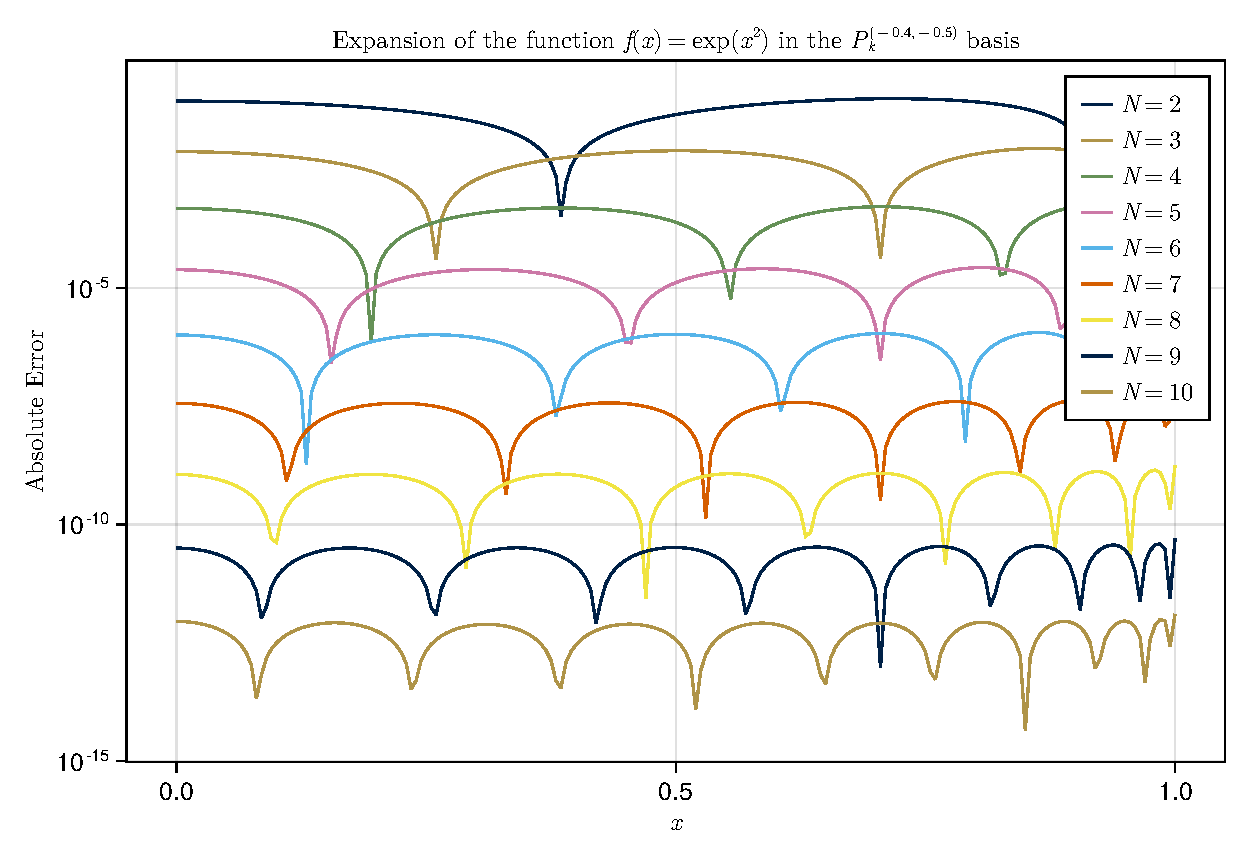
\includegraphics[width=0.75\linewidth]{results/jacobi-expansions.pdf}
  \caption[Convergence of Jacobi basis expansion]{Convergence of the Jacobi polynomial expansion $f_N(x) = \sum_{k=0}^{N-1} P_k^{(a, b)}(x)$ of an example function $f(x) = \e^{x^2}$ with $a = -\frac{3}{4}$ and $b = -\frac{1}{2}$. Each added term improves the absolute error between the function and its expansion by a factor, so we have exponential convergence. The number of ``arches'' of each solution error function, occurring from the roots of $f(x) - f_N(x)$, approximately equals the order $N$.}
  \label{fig:jacobi-expansions-error}
\end{figure}

An example of the approximation of a function using Jacobi polynomials is given in \Cref{fig:jacobi-expansions-error}, depicting the absolute error for expansions of growing order $N$.

As mentioned previously in \Cref{chap:particle-interaction-theory}, due to the absence of an external potential the solutions must be radially symmetric given that the pairwise interactions only depend on mutual distance and nothing else.
So in most upcoming instances, we will work with the \textit{radial} Jacobi polynomials, allowing us to extend the preimage of the polynomial basis from $\R$ to $\R^d$.
These are simply given by $\jacobi[k]{x}$.
